% E-Voting Machine © 2024 by S4Y Solutions is licensed under CC BY-NC-ND 4.0.
% To view a copy of this license, visit https://creativecommons.org/licenses/by-nc-nd/4.0/
\documentclass[12pt]{beamer}

% ****************
% ***** INFO *****
% ****************
\usepackage[english]{babel}
\title[Insitute]{e-Voting Machine}
\subtitle{Investor Presentation}
\author[Sergey Dolin]{Sergey Dolin \\
\href{mailto:sergey@s4y.solutions}{\scriptsize{sergey@s4y.solutions}} \\ }
\institute[Institute]{S4Y Solutions}
\newcommand{\prevyear}{\the\numexpr\year-1\relax} % \nextyear
\newcommand{\currentyear}{\the\year} % \currentyear
\date{\prevyear/\currentyear} % or \today

% *******************
% ***** PROJECT *****
% *******************
\usepackage{tikz-uml}

\definecolor{main}{HTML}{0000FF}
\setbeamercolor{structure}{fg=main}

\newcommand{\copyrightnote}{
    \vfill
    \begin{flushleft}
    \tiny
    E-Voting Machine \textcopyright \currentyear~by S4Y Solutions is licensed under \href{https://creativecommons.org/licenses/by-nc-nd/4.0}{CC BY-NC-ND 4.0.}
    %To view a copy of this license, visit \url{https://creativecommons.org/licenses/by-nc-nd/4.0/}
    \end{flushleft}
}

\addtobeamertemplate{footline}{%
    \copyrightnote
}

\tikzset{custom component/.style={
    minimum height=0.5em, % Adjust the height here
    text width=4em, % Adjust the text width if needed
    draw,
    fill=blue!20,
    font=\small
}}

% *****************
% ***** THEME *****
% *****************
\usetheme{Luebeck}
\usepackage{helvet}
\renewcommand{\familydefault}{\sfdefault}
\setbeamertemplate{frametitle continuation}{\gdef\beamer@frametitle{}}
\setbeamertemplate{footline}{}

% *****************
% ***** CODE *****
% *****************
\usepackage{listings}
\lstdefinestyle{java}{
    backgroundcolor=\color{white},
    basicstyle=\ttfamily\scriptsize,
    breaklines=true,
    commentstyle=\color{gray},
    keywordstyle=\color{blue},
    stringstyle=\color{magenta},
    identifierstyle=\color{black},
    numberstyle=\color{gray},
    language=Java
}
\lstdefinestyle{cpp}{
    backgroundcolor=\color{white},
    basicstyle=\ttfamily\scriptsize,
    breaklines=true,
    commentstyle=\color{gray},
    keywordstyle=\color{blue},
    stringstyle=\color{magenta},
    identifierstyle=\color{black},
    numberstyle=\color{gray},
    language=C++
}
\lstdefinestyle{py}{
    backgroundcolor=\color{white},
    basicstyle=\ttfamily\scriptsize,
    breaklines=true,
    commentstyle=\color{gray},
    keywordstyle=\color{blue},
    stringstyle=\color{magenta},
    language=Python
}
\lstdefinestyle{js}{
    backgroundcolor=\color{white},
    basicstyle=\ttfamily\scriptsize,
    breaklines=true,
    commentstyle=\color{gray},
    keywordstyle=\color{blue},
    stringstyle=\color{magenta},
    identifierstyle=\color{black},
    numberstyle=\color{gray},
    language=JavaScript,
    escapechar=@
}
\lstdefinestyle{sh}{
    basicstyle=\ttfamily\scriptsize,
    breaklines=true,
    commentstyle=\color{gray},
    keywordstyle=\color{blue},
    stringstyle=\color{magenta},
    identifierstyle=\color{black},
    numberstyle=\color{gray},
    language=bash
}

% **********************
% ***** ALGORITHMS *****
% **********************
\usepackage{algorithm}
\usepackage{algpseudocode}

% *****************
% ***** UTILS *****
% *****************
\usepackage{xcolor}
\usepackage{blkarray}

% ********************
% ***** DOCUMENT *****
% ********************
\begin{document}

% **********************
% ***** TITLEPAGE ******
% **********************
    \begin{frame}{}
        \vspace{\fill}

        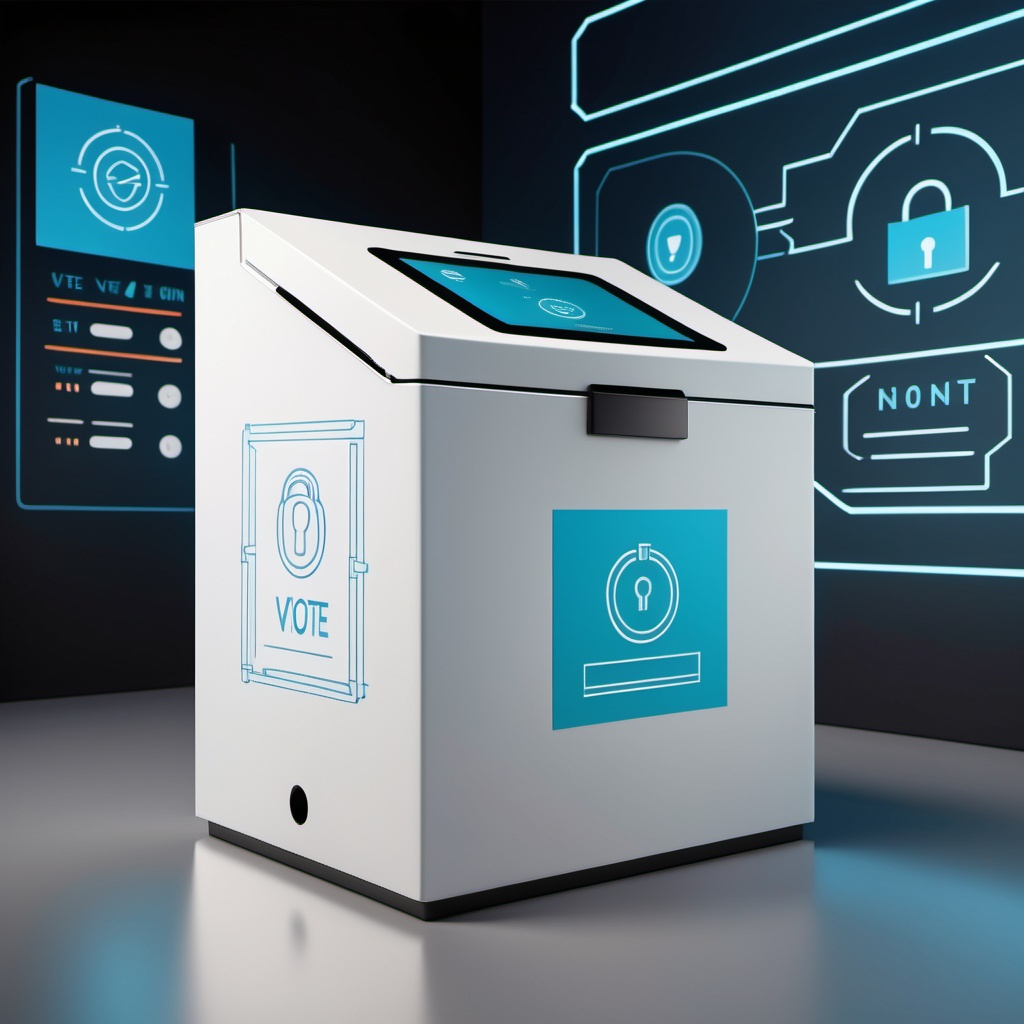
\includegraphics[width=0.16\linewidth]{voting-machine}

        \vspace{\fill}

        \Large
        \color{main}
        \inserttitle

        \medskip

        \large
        \color{black}
        \insertsubtitle

        \vspace{\fill}

        \footnotesize
        \insertinstitute

        \vspace{\fill}

        \textbf{Author:} \insertauthor

        \medskip

        \insertdate

        \vspace{\fill}
        \copyrightnote
    \end{frame}

% ********************
% ***** Problems *****
% ********************
    \begin{frame}[allowframebreaks]{The Challenges of the Voting Process}
        \vfill
        Voting presents two critical challenges:

        \begin{itemize}
            \item \textbf{Balancing Transparency and Privacy:} The need to verify each cast vote while maintaining the anonymity of the voter.
            \item \textbf{Voter Identification:} Ensuring that each voter is uniquely and securely identified.
        \end{itemize}
        \copyrightnote
    \end{frame}


% ***********************************
% ***** Transparency vs Privacy *****
% ***********************************
    \begin{frame}[allowframebreaks]{Transparency vs Privacy}
        \vfill
        \begin{block}{Unsolvable contradiction}
            The challenge of verifying a vote while maintaining complete privacy seems like an unsolvable contradiction
        \end{block}

        \begin{exampleblock}{Solution}
            Allowing voters to cast multiple votes lets them verify their choice while keeping the actual vote
            undiscoverable
        \end{exampleblock}

        \begin{alertblock}{Raises another problem}
            Allowing multiple votes opens the door for potential fraud
        \end{alertblock}
        \vfill
        \textbf{Revenue: Secure, Transparent Cast Ledger Service}
        \copyrightnote
    \end{frame}

% ********************************
% ***** Voter Identification *****
% ********************************
    \begin{frame}[allowframebreaks]{Voter Identification}
        \vfill

        \begin{block}{Conventional Voting}
            Paper ballots does not solve the problem of the identification completely
        \end{block}

        \begin{exampleblock}{e-Voting}
            Neither e-voting can identify a voter with absolute certainty, due to the limitations in accessing personal
            data, but it is possible to provide a predictable level of certainty with different built-in and external
            services
        \end{exampleblock}
        \vfill
        \textbf{Revenue: Paid identification services}\\
        \scriptsize{\textit{(emails, biometric, heuristic, government and NGO-issued IDs, etc)}}

        \copyrightnote
    \end{frame}

% **********************************
% ***** e-Voting Vulnarability *****
% **********************************
    \begin{frame}[allowframebreaks]{e-Voting Specific Vulnerability}
        \vfill
        \begin{block}{Conventional Voting}
            The voting booth provides a level of protection against external influence on how the voter casts their vote.
        \end{block}

        \begin{alertblock}{e-Voting}
            In electronic voting, it is impossible to protect the voter from being forced to vote in a specific way.
        \end{alertblock}

        \begin{exampleblock}{Multiple Voting}
            Multiple voting allows the voter to cast their vote freely, without external pressure
        \end{exampleblock}

        \copyrightnote
    \end{frame}

% **************************
% ***** Extra benefits *****
% **************************
    \begin{frame}[allowframebreaks]{Extra benefits}
        \vfill
        Supplementary and Related Services:
        \begin{itemize}
            \item \textbf{Real-time Vote Tally:} Exit-polling Service
            \item \textbf{Historical data:} API to access historical voting data
            \item \textbf{Extra security:} Provide services with private access
        \end{itemize}
        \copyrightnote
    \end{frame}

% *******************
% ***** Ledgers *****
% *******************
    \begin{frame}[allowframebreaks]{Implementation details: Ledgers}
        \vfill
        \begin{block}{Altering votes issue}
            Allowing vote alterations implies modifications to records, which can undermine trust
            in the service.
        \end{block}

        \begin{exampleblock}{Immutable ledger}
            This is addressed by an add-only ledger and a two-step vote change: negating the old
            vote and casting a new one.
        \end{exampleblock}

        \begin{alertblock}{Raises another problem}
            Consequence votes introduce the need to link back to the previous vote, which compromises
            voter anonymity as it can be traced.
        \end{alertblock}

        \copyrightnote
    \end{frame}

% ***************************
% ***** Smart contracts *****
% ***************************
    \begin{frame}[allowframebreaks]{Implementation details: Smart contracts}
        \vfill
        \begin{block}{Don't keep the link to the previous vote}
            It is not necessary to link to the previous vote in order to negate it.
            Regardless of when or who cast the vote, simply knowing which vote it was
            and adding its negation to the ledger will effectively remove the previous vote.
        \end{block}
        \begin{exampleblock}{Voting with deffered self-contained code snippet}
            Smart contracts are chosen for this purpose—these are secured, signed code snippets
            executed in an isolated environment.
            This approach was selected due it fits well with existing infrastructure and industry
            standards, making it both practical and reliable.
        \end{exampleblock}
        \copyrightnote
    \end{frame}

% ****************************
% ***** Process overview *****
% ****************************
    \tikzumlset{font=\scriptsize}
    \begin{frame}[allowframebreaks]{High-level overview of the voting flow}
        \vfill
        \begin{center}
            \begin{tikzpicture}
                \begin{umlseqdiag}
                    \umlactor[no ddots, scale=0.4]{Voter}
                    \umlactor[no ddots, scale=0.4, x = 2]{Voting Owner}
                    \umldatabase[no ddots, scale=0.6, x = 4.5]{Voters Registry}
                    \umlmulti[no ddots, scale=0.4, x = 7]{Cast Ledger}
                    \begin{umlcall}[op={create voting}, dt = 3]{Voting Owner}{Voters Registry}
                    \end{umlcall}
                    \begin{umlcall}[op={request ballot}, dt = 8.5, return=smart contract(yes/no)]{Voter}{Voters Registry}
                    \end{umlcall}
                    \begin{umlcall}
                        [op={apply contract(yes\textbar no)}, dt = 4, return=smart contract(yes/no) and cast ID]{Voter}{Cast Ledger}
                    \end{umlcall}
                \end{umlseqdiag}
            \end{tikzpicture}
        \end{center}
        \copyrightnote
    \end{frame}

% ************************************
% ***** Ensuring trust in voting *****
% ************************************

    \begin{frame}[allowframebreaks]{Ensuring trust in voting}
        \vfill
        Transparency is the key to ensuring trust in the voting process.
        \begin{itemize}
            \item \textbf{Voters Registry:} Shows only the issuance of ballots without linking
            votes to individual voters
            \item \textbf{Cast Ledger and Issued Contracts Ledgers:} Make it possible to
            verify only system issued ballots were used for voting
            \item \textbf{Open Smart Contract Code:} Since no code other than the
            smart contract can affect the voting process, it ensures trustworthiness in e-voting
            \item \textbf{3rd Party Provided Ledgers:} Hosting the ledgers and running
            smart contracts on public blockchains eliminates doubts about data tampering
        \end{itemize}
        \copyrightnote
    \end{frame}

% *************************
% ***** More security *****
% *************************

    \begin{frame}[allowframebreaks]{Enhancing Security}
        \vfill
        Moderate level of security assumes that each cast (or applying the smart contract) has
        its own unique ID, allowing voters to verify that their vote is recorded in the ledger.

        Each vote has a unique ID, so the voter can confirm his vote was counted. While
        this ID doesn’t reveal which specific vote he made (since he can vote multiple
        times), seeing that a new vote was cast suggests he might have changed
        his mind.

        It’s possible to offer a service with anonymous contracts. However, this means
        no one can verify a specific vote, so both the smart contracts and ledgers
        must be completely trustworthy.
        \copyrightnote
    \end{frame}

% **************************
% ***** Infrastructure *****
% **************************
    \begin{frame}[allowframebreaks]{Implementation details: Infrastucture}
        \vfill
        The terms “Smart Contracts” and “Ledgers” might suggest the system relies on blockchain technology.
        While blockchain is a suitable option, it’s not the only one. The system can also be implemented with
        a traditional, audited database or a secure cloud-hosted server.

        Even if blockchain is used, it doesn’t have to be public. A self-hosted, private blockchain could be
        considered in the actual implementation.
        \copyrightnote
    \end{frame}

% *********************************
% ***** Voters identification *****
% *********************************
    \begin{frame}[allowframebreaks]{Implementation details: Voters identifications}
        \vfill
        Although this presentation focuses on the voting process, the initial stage of issuing ballots is crucial.

        It is not covered here because it will be implemented as a separate service. This service will support plugins
        and be extendable based on client needs and available data sources.
        \copyrightnote
    \end{frame}

% *************************
% ***** Microservices *****
% *************************
    \begin{frame}[allowframebreaks]{Implementation details: Microservices}
        \vfill
        The system should be built from loosely coupled microservices connected by a common protocol,
        allowing components to be swapped based on client needs.
        \copyrightnote
    \end{frame}


% **************************
% ***** Current status *****
% **************************
    \begin{frame}[allowframebreaks]{Current status}
        \vfill
        At the time of writing, the project includes a Proof of Concept Lua-based reference
        implementation available in a public repository on
        GitHub: \url{https://github.com/s4ysolutions/e-voting-machine}.
        \copyrightnote
    \end{frame}
\end{document}